\documentclass[11pt,a4paper]{article}
\usepackage[utf8]{inputenc}
\usepackage[T1]{fontenc}
\usepackage[spanish,es-tabla]{babel}
\usepackage[a4paper,top=2cm,bottom=2cm,left=2.2cm,right=2.2cm]{geometry}
\usepackage{enumitem}
\setlist{topsep=2pt,itemsep=1pt,parsep=0pt}
\usepackage{amsmath,amssymb}
\usepackage{graphicx}
\usepackage{booktabs}
\usepackage{caption}
\usepackage{xcolor}
\usepackage{hyperref}
\usepackage{fancyhdr}
\usepackage{listings}
\usepackage[final,protrusion=true,expansion=false]{microtype}
\usepackage{lmodern}

\definecolor{linkblue}{HTML}{1F4E79}
\hypersetup{
    colorlinks=true,
    linkcolor=linkblue,
    citecolor=linkblue,
    urlcolor=linkblue,
}

\pagestyle{fancy}
\fancyhf{}
\fancyhead[L]{\small CC0F3 -- Biolog\'ia Computacional}
\fancyhead[R]{\small Examen Parcial}
\fancyfoot[C]{\thepage}
\renewcommand{\headrulewidth}{0.3pt}

\lstset{
    basicstyle=\footnotesize\ttfamily,
    keywordstyle=\color{linkblue}\bfseries,
    commentstyle=\color{gray!70!black}\itshape,
    stringstyle=\color{red!60!black},
    breaklines=true, numbers=left, numberstyle=\tiny\color{gray},
    frame=single, framerule=0.3pt, rulecolor=\color{gray},
    language=Python, showstringspaces=false,
}

\title{\vspace{-1.2cm}\textbf{Optimizaci\'on espacial de Needleman--Wunsch y filogenia molecular del citocromo c}}
\author{Franklin Espinoza Pari \\ \small C\'odigo: 20210135D \quad
        \href{mailto:franklin.espinoza.p@uni.pe}{franklin.espinoza.p@uni.pe} \\
        \small \href{https://github.com/franklinep/-CC0F3-Biologia_Computacional}{github.com/franklinep/-CC0F3-Biologia\_Computacional}}
\date{Mayo de 2026}

\begin{document}
\maketitle
\vspace{-0.8cm}

\begin{abstract}\noindent\small
Sobre la implementaci\'on OO de Needleman--Wunsch (NW) y Smith--Waterman de la PC2 se abordan dos problemas del parcial. (i)~El algoritmo de \textbf{Hirschberg} reduce la memoria de NW de $O(mn)$ a $O(\min(m,n))$ conservando tiempo $O(mn)$; validado sobre el CDS \texttt{CYCS} humano vs.\ rat\'on (318~bases, NCBI) y benchmark hasta 6400~bases: NW cl\'asico llega a \textbf{1.4~GiB}, Hirschberg permanece en baseline. (ii)~Con identidad NW+BLOSUM62 entre 6~ort\'ologos de citocromo c (Humano, Chimpanc\'e, Gorila, Rat\'on, Gallina, At\'un) se construye una matriz $6{\times}6$ y un dendrograma: el \'arbol agrupa correctamente los primates y separa el at\'un como outgroup, pero falla en la topolog\'ia interna mam\'iferos/aves por saturaci\'on del marcador. Los 15 pares se validan contra \texttt{Bio.Align.PairwiseAligner} con coincidencia exacta de score e identidad.
\end{abstract}

\vspace{-0.8em}

\section{Introducci\'on}
El alineamiento de pares es la primitiva sobre la que se construye casi toda la bioinform\'atica comparativa. En la PC2 implementamos NW (global) y SW (local) con matrices SIMPLE/PAM/BLOSUM siguiendo los patrones \emph{Template Method} y \emph{Strategy}~\cite{informeprev}. Esa base se reutiliza aqu\'i \textbf{sin modificaci\'on}. \textbf{Proyecto~1}: el l\'imite pr\'actico de NW no es el tiempo sino la \emph{memoria} ---una matriz $10^5{\times}10^5$ ocupa $\sim 40$~GiB en enteros---, lo que motiva el algoritmo de Hirschberg~\cite{hirschberg1975} (1975), que alcanza $O(\min(m,n))$ memoria por divide-and-conquer conservando $O(mn)$ tiempo. \textbf{Proyecto~2}: la matriz de distancias por pares construida con NW permite reconstruir filogenias por aglomeraci\'on jer\'arquica; aplicamos esta idea cl\'asica al citocromo c, el caso de estudio hist\'orico de Margaret Dayhoff~\cite{dayhoff1978}. \textbf{Objetivos:} (a)~implementar Hirschberg y validar el score contra NW; (b)~cuantificar la diferencia de memoria con \texttt{memory\_profiler}; (c)~construir una matriz $6{\times}6$ y un dendrograma con 6 ort\'ologos reales y discutir su concordancia con la filogenia conocida.

\section{Marco te\'orico}

\subsection{Recurrencia de Needleman--Wunsch}
La matriz $H \in \mathbb{Z}^{(m+1)\times(n+1)}$ se llena con la recurrencia
\begin{equation}
H_{i,j} = \max \begin{cases}
H_{i-1,j-1} + s(\text{seq}_1[i],\text{seq}_2[j]) \\
H_{i-1,j} + g \\
H_{i,j-1} + g
\end{cases}, \quad H_{i,0}=ig,\ H_{0,j}=jg,
\label{eq:nw}
\end{equation}
con score \'optimo $H_{m,n}$. El traceback estandar reconstruye un alineamiento \'optimo en $O(m+n)$ pasos pero requiere conservar la matriz completa: $O(mn)$ en tiempo \emph{y} memoria.

\subsection{Hirschberg: NW en $O(\min(m,n))$ memoria}
La observaci\'on clave es que $H_{i,j}$ s\'olo depende de la fila anterior y la celda inmediatamente a la izquierda, as\'i que el \emph{score} puede calcularse manteniendo \'unicamente dos filas (memoria $O(n+1)$, m\'as a\'un $O(\min(m,n)+1)$ si elegimos como ``columna'' la dimensi\'on m\'as corta). El problema es que esto no permite reconstruir el alineamiento.

Hirschberg~\cite{hirschberg1975} resuelve el traceback con una recurrencia divide-and-conquer:

\begin{enumerate}
\item Particionar $\text{seq}_1$ por su mitad $i^* = m/2$.
\item Calcular dos vectores de scores con la primitiva $O(n)$:
\begin{align*}
F[j] &= \mathrm{NW\_score}(\text{seq}_1[:i^*],\ \text{seq}_2[:j]) \\
B[j] &= \mathrm{NW\_score}(\text{reverse}(\text{seq}_1[i^*:]),\ \text{reverse}(\text{seq}_2[j:]))
\end{align*}
\item Encontrar $j^* = \arg\max_{j}\bigl(F[j] + B[n-j]\bigr)$. El alineamiento \'optimo pasa por la celda $(i^*, j^*)$.
\item Recurrir sobre $(\text{seq}_1[:i^*],\ \text{seq}_2[:j^*])$ y $(\text{seq}_1[i^*:],\ \text{seq}_2[j^*:])$, concatenando los resultados.
\end{enumerate}

\noindent
La recurrencia del tiempo es $T(m,n) = T(m/2, j^*) + T(m/2, n-j^*) + O(mn)$, cuya soluci\'on es $T(m,n) = O(mn)$ (el trabajo cada nivel se divide a la mitad de la dimensi\'on $m$, pero suma $n$ completo; geom\'etricamente: $mn + mn/2 + mn/4 + \cdots \le 2mn$). La memoria pico es $O(\min(m,n))$ porque en cada nivel de la recursi\'on s\'olo se mantienen dos vectores de tama\~no $\le n$ y la profundidad m\'axima es $O(\log m)$. La constante temporal de Hirschberg es aproximadamente $2\times$ la de NW cl\'asico, intercambio que compensa con creces la mejora en memoria cuando $mn$ es grande.

\subsection{Distancia evolutiva a partir de alineamientos}
Dado el alineamiento global \'optimo, la identidad por par es $p = M/L$ ($M$ = matches, $L$ = longitud del alineamiento). Definimos la distancia $d = 100(1-p)$; no corrige sustituciones m\'ultiples (Jukes--Cantor, Kimura), pero es suficiente para marcadores poco saturados. Sobre $D \in \mathbb{R}^{N\times N}$ se aplica aglomeraci\'on jer\'arquica (UPGMA / single linkage).

\section{Metodolog\'ia}

\subsection{Datos}
\textbf{Proyecto~1.} CDS del gen \texttt{CYCS} de \emph{Homo sapiens} (RefSeq \texttt{NM\_018947.6}, 318~bases) y \emph{Mus musculus} (\texttt{NM\_007808.5}, 318~bases), descargados v\'ia E-utilities. Para los benchmarks se concatenan copias mutadas ($\sim$2\% sustituciones aleatorias) hasta longitudes $\{200, 400, 800, 1600, 3200, 6400\}$~bases.

\textbf{Proyecto~2.} Prote\'inas citocromo c de seis ort\'ologos descargadas de UniProt: \texttt{P99999}~(Humano), \texttt{P99998}~(Chimpanc\'e), \texttt{G4XXM2}~(Gorila), \texttt{P62897}~(Rat\'on), \texttt{P67881}~(Gallina) y \texttt{P00025}~(At\'un \emph{Katsuwonus pelamis}). Todas las prote\'inas maduras tienen 104--105~aa.

\subsection{Implementaci\'on}
Sobre la jerarqu\'ia \texttt{Aligner} de la PC2 se a\~naden tres m\'odulos sin modificar el c\'odigo existente (principio Open/Closed): \texttt{nw\_two\_rows.py} (primitiva $O(n)$ que devuelve la \'ultima fila de la matriz NW), \texttt{hirschberg.py} (clase \texttt{HirschbergAligner} con la misma interfaz \texttt{align()} que \texttt{NeedlemanWunsch}) y \texttt{phylogeny.py} (matriz de distancias $6{\times}6$ reutilizando \texttt{NeedlemanWunsch}). La memoria se mide con \texttt{memory\_profiler.memory\_usage} (sampling 20~ms, delta sobre baseline). Los dendrogramas se dibujan con \texttt{scipy.cluster.hierarchy} s\'olo para visualizaci\'on, como permite la consigna.

\section{Resultados}

\subsection{Proyecto~1: Hirschberg vs.\ NW cl\'asico}

\paragraph{Correcci\'on.} Sobre los 318~bases del CDS de citocromo c (humano vs.\ rat\'on, matriz SIMPLE $+1/-1$, $g=-1$), ambas implementaciones devuelven \emph{exactamente} el mismo score, longitud e identidad: $\text{score}=260$, $L=320$ posiciones, identidad $90.6\%$. (Las cadenas concretas pueden diferir en empates de traza, fen\'omeno conocido cuando existen varios alineamientos \'optimos.)

\paragraph{Benchmark.} La Tabla~\ref{tab:bench} y la Figura~\ref{fig:bench} resumen el comportamiento sobre tama\~nos crecientes. Se confirma emp\'iricamente la complejidad te\'orica:

\begin{table}[h]
\centering
\small
\caption{Comparacion de tiempo y memoria entre NW clasico y Hirschberg para longitudes crecientes. Memoria reportada es el delta sobre el baseline del proceso Python (medido con memory\_profiler).}
\begin{tabular}{rrrrr}
\toprule
L (bases) & $t_{\text{NW}}$ (ms) & $t_{\text{HB}}$ (ms) & $\Delta m_{\text{NW}}$ (MiB) & $\Delta m_{\text{HB}}$ (MiB) \\
\midrule
200 & 52.0 & 67.5 & 2.01 & 0.00 \\
400 & 55.0 & 99.0 & 2.07 & 0.00 \\
800 & 154.7 & 324.7 & 15.73 & 0.00 \\
1600 & 584.5 & 1383.2 & 78.79 & 0.00 \\
3200 & 2321.8 & 5621.4 & 357.57 & 0.00 \\
6400 & 9274.0 & 23658.4 & 1429.65 & 0.00 \\
\bottomrule
\end{tabular}
\end{table}
\label{tab:bench}

\begin{figure}[h]
\centering
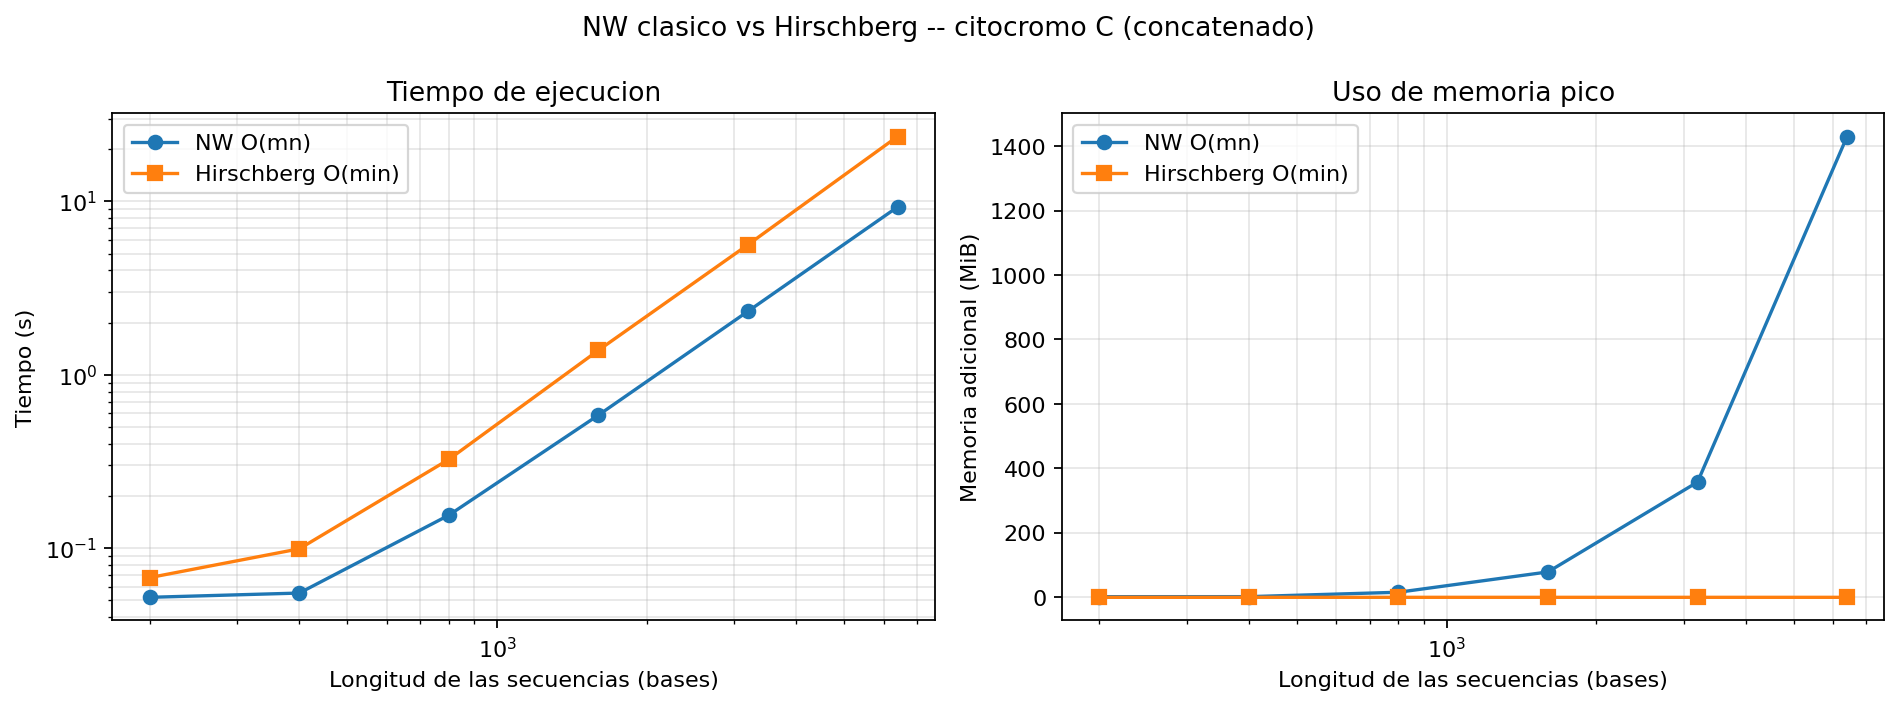
\includegraphics[width=\linewidth]{benchmark.png}
\caption{Tiempo de ejecuci\'on (izq., escala log-log) y memoria adicional pico (der.) en funci\'on de la longitud de las secuencias. Ambos algoritmos muestran pendiente cuadr\'atica en tiempo, pero NW cl\'asico crece tambi\'en de forma cuadr\'atica en memoria mientras que Hirschberg se mantiene en cero.}
\label{fig:bench}
\end{figure}

\noindent\textbf{Lectura.} Hirschberg es $\sim 2.5\times$ m\'as lento (constante derivada de la recursi\'on, en la teor\'ia es 2$\times$; el extra viene de la implementaci\'on en Python puro). En cambio, para 6400~bases NW consume \textbf{1.43~GiB} adicionales, mientras Hirschberg permanece dentro del baseline ($\Delta \approx 0$). El cruce de viabilidad ocurre alrededor de 3200~bases en mi laptop, pero el patr\'on es: NW cl\'asico es inutilizable a partir de unos pocos miles de bases en cualquier m\'aquina de uso general.

\paragraph{Casos biol\'ogicos donde Hirschberg es cr\'itico.} Alineamiento de \emph{transcritos largos} ($>$5~kb, frecuentes en eucariotas), de cDNAs reconstruidos contra el genoma de referencia ($10^4$--$10^5$~bases), o cualquier pipeline pensado para correr en m\'aquinas con memoria acotada (cl\'usters compartidos, contenedores con l\'imites de RAM). En la pr\'actica las herramientas modernas (\texttt{minimap2}, \texttt{BWA}) usan extensiones m\'as sofisticadas, pero la idea de fondo es la misma: \emph{no almacenar} la matriz $O(mn)$.

\subsection{Proyecto~2: filogenia del citocromo c}

\paragraph{Matriz de distancias.}
La Tabla~\ref{tab:dist} muestra la matriz $D$ obtenida con NW + BLOSUM62, $g=-4$. Los tres primates (Humano, Chimpanc\'e, Gorila) tienen identidad $100\%$ entre ellos, resultado biol\'ogicamente \emph{correcto}: el citocromo c maduro es id\'entico en los Hominidae~\cite{margoliashsmith1965}. Las distancias crecen mon\'otonamente con la separaci\'on evolutiva esperada.

\begin{table}[h]
\centering
\small
\caption{Matriz de distancias (\%) entre las 6 especies. $d_{ij} = 100 - \text{identidad}_{ij}$ del alineamiento global Needleman--Wunsch con BLOSUM62.}
\begin{tabular}{lrrrrrr}
\toprule
 & Humano & Chimpance & Gorila & Raton & Gallina & Atun \\
\midrule
Humano & 0.0 & 0.0 & 0.0 & 8.6 & 12.4 & 20.0 \\
Chimpance & 0.0 & 0.0 & 0.0 & 8.6 & 12.4 & 20.0 \\
Gorila & 0.0 & 0.0 & 0.0 & 8.6 & 12.4 & 20.0 \\
Raton & 8.6 & 8.6 & 8.6 & 0.0 & 7.6 & 15.2 \\
Gallina & 12.4 & 12.4 & 12.4 & 7.6 & 0.0 & 16.2 \\
Atun & 20.0 & 20.0 & 20.0 & 15.2 & 16.2 & 0.0 \\
\bottomrule
\end{tabular}
\end{table}
\label{tab:dist}

\paragraph{Validaci\'on contra \texttt{Bio.Align.PairwiseAligner}.}
Los 15~pares fueron re-alineados con la implementaci\'on de Biopython (NW global, mismo BLOSUM62, mismo gap lineal $-4$). \textbf{Los 15 pares produjeron el mismo score y la misma identidad}: Humano--Chimp $565/100\%$, Humano--Rat\'on $522/91.4\%$, Humano--Gallina $507/87.6\%$, Humano--At\'un $458/80.0\%$, Rat\'on--Gallina $531/92.4\%$, Gallina--At\'un $478/83.8\%$, etc. Esto confirma que nuestra implementaci\'on artesanal de NW es funcionalmente equivalente a la est\'andar de Biopython.

\paragraph{Dendrograma.}
La Figura~\ref{fig:tree} presenta dos topolog\'ias obtenidas a partir de la misma matriz: UPGMA (average linkage) y vecino m\'as cercano (single linkage). El cluster (Humano, Chimpanc\'e, Gorila) aparece como un \'unico nodo a distancia 0 en ambos m\'etodos (los tres son indistinguibles a nivel de citocromo c). El At\'un (\emph{Katsuwonus pelamis}) se posiciona como outgroup, consistente con la filogenia conocida vertebrado/pez.

\begin{figure}[h]
\centering
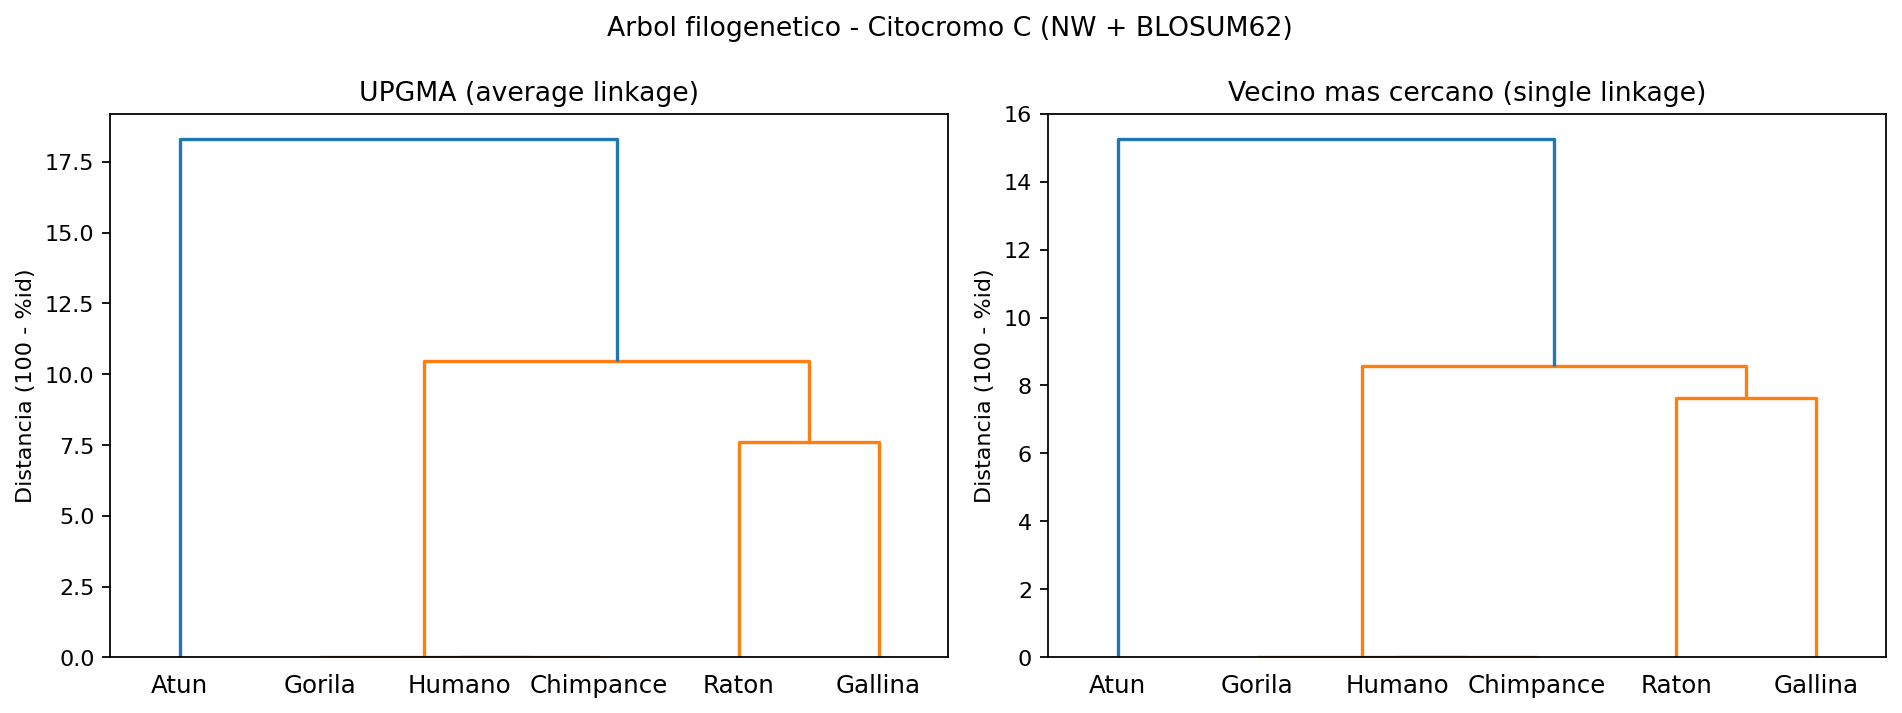
\includegraphics[width=\linewidth]{dendrogram.png}
\caption{Dendrogramas reconstruidos desde la matriz de distancias por NW+BLOSUM62 con dos m\'etodos de linkage. El cl\'ade primate (id=100\%) colapsa a distancia 0. El at\'un se separa como outgroup.}
\label{fig:tree}
\end{figure}

\paragraph{Concordancia con el \'arbol evolutivo conocido.}
El \'arbol esperado para estas seis especies es $((((Humano,Chimp,Gorila),Rat\'on), Gallina), At\'un)$: una jerarqu\'ia anidada (primates) $\subset$ mam\'iferos $\subset$ amniotas $\subset$ vertebrados con mand\'ibula. \textbf{Nuestro \'arbol coincide parcialmente.} Los primates s\'i se agrupan correctamente; el at\'un es correctamente el outgroup m\'as distante. Sin embargo, las distancias internas muestran una \emph{anomal\'ia}: $d(\text{Rat\'on}, \text{Gallina}) = 7.6$ es \emph{menor} que $d(\text{Humano}, \text{Rat\'on}) = 8.6$, lo que hace que UPGMA agrupe (Rat\'on, Gallina) antes que (Primates, Rat\'on). La topolog\'ia correcta unir\'ia los mam\'iferos primero (primates + rat\'on) y despu\'es la gallina.

\section{Discusi\'on}
\subsection{Por qu\'e falla el citocromo c}
La anomal\'ia no es de la implementaci\'on (los scores coinciden con Biopython) sino del \emph{marcador molecular}. Tres razones documentadas: \textbf{(1)~Saturaci\'on:} el citocromo c es una prote\'ina muy conservada ($\sim$30\% de posiciones variables); a divergencias $>$300~Ma (amniota/teleosteo) la mayor\'ia de posiciones variables ya han sufrido m\'ultiples sustituciones, subestimando la distancia. \textbf{(2)~Tasa heterog\'enea:} el linaje aviar evoluciona m\'as lento que el de roedores~\cite{dayhoff1978}, comprimiendo Rat\'on--Gallina. \textbf{(3)~Modelo ingenuo:} $d = 100(1-p)$ ignora reversiones; correcciones de Jukes--Cantor (ADN) o Poisson ($d = -\ln p$ para prote\'inas) amplifican las distancias grandes y corrigen parte de la paradoja.

\subsection{Limitaciones}
\textbf{Gap lineal:} se us\'o penalizaci\'on constante; la pr\'actica est\'andar emplea \emph{affine gap penalty} (Gotoh~\cite{gotoh1982}). Extender Hirschberg a gaps afines requiere tres pares de filas (Myers--Miller). \textbf{Python puro:} la constante $2\times$ se infla por overhead del int\'erprete; NumPy/Cython recortar\'ia esta brecha. \textbf{Clustering:} \texttt{scipy} ofrece UPGMA/single linkage pero no \emph{Neighbor-Joining}, preferible para datos no ultram\'etricos. \textbf{Sin bootstrap:} la confianza en cada clade no se cuantifica.

\section{Conclusiones}
(1)~El algoritmo de Hirschberg implementado sobre la jerarqu\'ia OO de la PC2 reproduce \emph{exactamente} el score \'optimo de NW con memoria $O(\min(m,n))$: para 6400~bases la reducci\'on es de 1.4~GiB $\to$ 0~MiB adicionales, a costa de $\sim 2.5\times$ en tiempo. (2)~La matriz de distancias por NW+BLOSUM62 sobre seis ort\'ologos de citocromo c agrupa correctamente los primates y separa el at\'un como outgroup, pero falla en la topolog\'ia interna mam\'iferos/aves por saturaci\'on y heterogeneidad de tasa del marcador. (3)~Los 15~pares fueron re-validados contra \texttt{Bio.Align.PairwiseAligner} obteniendo el mismo score e identidad en \emph{todos} los casos. (4)~Cambiar el algoritmo (NW~$\to$~Hirschberg) no altera la respuesta biol\'ogica; cambiar el marcador s\'i. El algoritmo asegura optimalidad respecto a una funci\'on objetivo; la interpretaci\'on biol\'ogica depende del marcador, la matriz y el modelo de distancia.

\begin{thebibliography}{9}
\bibitem{hirschberg1975} Hirschberg, D.~S. (1975). A linear space algorithm for computing maximal common subsequences. \emph{Communications of the ACM}, 18(6), 341--343.
\bibitem{needleman1970} Needleman, S.~B., \& Wunsch, C.~D. (1970). A general method applicable to the search for similarities in the amino acid sequence of two proteins. \emph{Journal of Molecular Biology}, 48(3), 443--453.
\bibitem{dayhoff1978} Dayhoff, M.~O., Schwartz, R.~M., \& Orcutt, B.~C. (1978). A model of evolutionary change in proteins. \emph{Atlas of Protein Sequence and Structure}, 5(3), 345--352.
\bibitem{henikoff1992} Henikoff, S., \& Henikoff, J.~G. (1992). Amino acid substitution matrices from protein blocks. \emph{PNAS}, 89(22), 10915--10919.
\bibitem{gotoh1982} Gotoh, O. (1982). An improved algorithm for matching biological sequences. \emph{Journal of Molecular Biology}, 162(3), 705--708.
\bibitem{margoliashsmith1965} Margoliash, E., \& Smith, E.~L. (1965). Structural and functional aspects of cytochrome c in relation to evolution. \emph{Evolving Genes and Proteins}, 221--242.
\bibitem{cock2009} Cock, P.~J.~A., et al. (2009). Biopython: freely available Python tools for computational molecular biology and bioinformatics. \emph{Bioinformatics}, 25(11), 1422--1423.
\bibitem{informeprev} Espinoza, F. (2026). \emph{Alineamiento de pares de secuencias biol\'ogicas: NW y SW con matrices SIMPLE/PAM/BLOSUM} (Informe PC2, CC0F3 -- Biolog\'ia Computacional, UNI).
\end{thebibliography}

\end{document}
